\subsection{Two Factors}

In figure \ref{fig:TrialDivisionGrowingprimesbits}, the default Trial Division algorithm shows total time taken to factorize a number consisting of two to 31 bits. In the figure \ref{fig:TrialDivisionGrowingprimes(modified:True)bits} the modified version of Trial Division can be seen.


\begin{figure}[H]
\centering
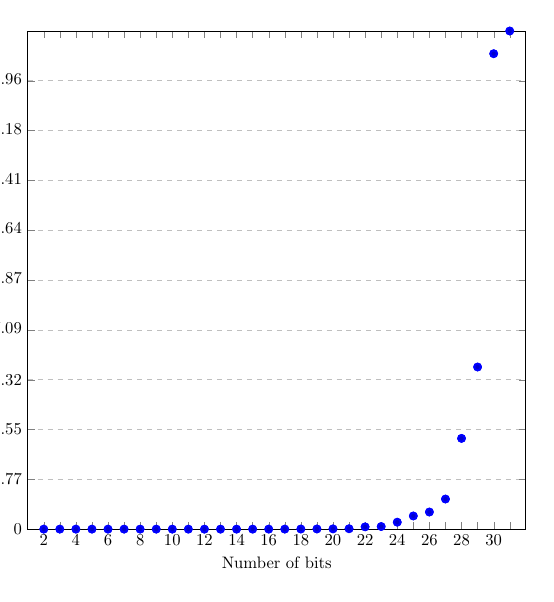
\begin{tikzpicture}[scale=0.6, trim axis left, trim axis right]
\begin{axis}[
    width=1\textwidth,
    height=1\textwidth,
    xlabel={Number of bits},
    ylabel={Time taken (s)},
    xmin=1.0, xmax=32.0,
    ymin=2.5e-05, ymax=3317.729958,
    xticklabels={2, , 4, , 6, , 8, , 10, , 12, , 14, , 16, , 18, , 20, , 22, , 24, , 26, , 28, , 30},
    xtick={2, 3, 4, 5, 6, 7, 8, 9, 10, 11, 12, 13, 14, 15, 16, 17, 18, 19, 20, 21, 22, 23, 24, 25, 26, 27, 28, 29, 30, 31},
    ytick={2.5e-05, 331.7730183, 663.5460116, 995.3190049, 1327.0919982, 1658.8649915, 1990.6379848, 2322.4109781, 2654.1839714, 2985.9569647},
    ymajorgrids=true,
    grid style=dashed,
]

\addplot+[
    blue,
    very thick,
    forget plot,
    only marks
    ]
    plot[
    very thick,
    error bars/.cd,
    y dir=plus,
    y explicit
    ]
    table[x=x,y=y,y error expr=\thisrow{y-max}] {
    x    y    y-max
    24	46.343519	0.303535
25	87.671617	0.0
26	114.011857	0.0
27	200.506368	0.0
20	1.7816451	0.0099209
21	2.7334088	0.0124842
22	15.1897874	0.0405596
23	17.2848708	0.0968762
28	604.359222	0.0
29	1079.771318	0.0
3	3.6e-05	1e-06
2	9.92e-05	0.0006538
5	9.65e-05	8.5e-06
4	6.69e-05	1.1e-06
7	0.0002478	2.52e-05
6	0.0001303	1.17e-05
9	0.0008995	1.35e-05
8	0.0003846	5.4e-06
11	0.0022981	4.79e-05
10	0.0016313	8.7e-06
13	0.0202252	0.0139458
12	0.0112163	0.0006427
15	0.0520107	0.0003753
14	0.0293946	0.0005424
17	0.204421	0.02304
16	0.1269137	0.0005663
19	1.1880814	0.0064836
18	0.8096179	0.0320171
31	3317.729958	0.0
30	3166.677136	0.0

    };

\addplot+[
    blue,
    very thick,
    forget plot,
    only marks
    ]
    plot[
    very thick,
    error bars/.cd,
    y dir=plus,
    y explicit
    ]
    table[x=x,y=y,y error expr=\thisrow{y-min}] {
    x    y    y-min
    24	46.343519	-0.204036
25	87.671617	0.0
26	114.011857	0.0
27	200.506368	0.0
20	1.7816451	-0.0146871
21	2.7334088	-0.0110068
22	15.1897874	-0.0581414
23	17.2848708	-0.0764928
28	604.359222	0.0
29	1079.771318	0.0
3	3.6e-05	-1e-06
2	9.92e-05	-7.42e-05
5	9.65e-05	-1.5e-06
4	6.69e-05	-9e-07
7	0.0002478	-2.8e-06
6	0.0001303	-4.3e-06
9	0.0008995	-4.5e-06
8	0.0003846	-1.6e-06
11	0.0022981	-2.11e-05
10	0.0016313	-1.03e-05
13	0.0202252	-0.0031632
12	0.0112163	-0.0001823
15	0.0520107	-0.0005167
14	0.0293946	-0.0003306
17	0.204421	-0.004761
16	0.1269137	-0.0005107
19	1.1880814	-0.0035704
18	0.8096179	-0.0088229
31	3317.729958	0.0
30	3166.677136	0.0

    };

\end{axis}
\end{tikzpicture}
\vspace{-0.3cm}
\caption{Factors between 2 and 31 bits}\label{fig:TrialDivisionGrowingprimesbits}
\end{figure}




\begin{figure}[H]
\centering
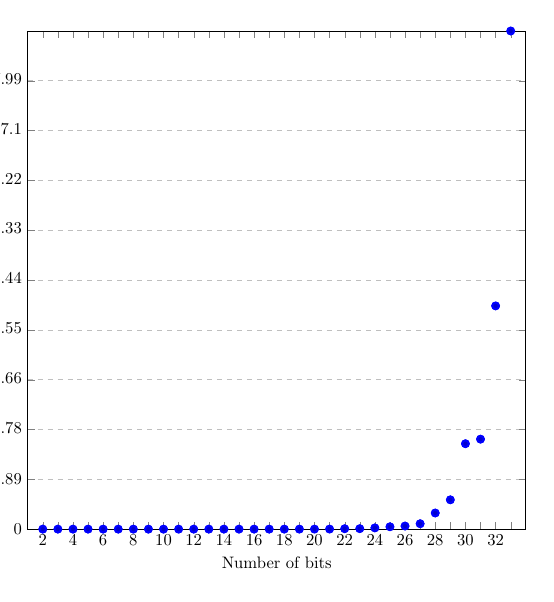
\begin{tikzpicture}[scale=0.6, trim axis left, trim axis right]
\begin{axis}[
    width=1\textwidth,
    height=1\textwidth,
    xlabel={Number of bits},
    ylabel={Time taken (s)},
    xmin=1.0, xmax=34.0,
    ymin=2.1e-05, ymax=9208.879762,
    xticklabels={2, , 4, , 6, , 8, , 10, , 12, , 14, , 16, , 18, , 20, , 22, , 24, , 26, , 28, , 30, , 32},
    xtick={2, 3, 4, 5, 6, 7, 8, 9, 10, 11, 12, 13, 14, 15, 16, 17, 18, 19, 20, 21, 22, 23, 24, 25, 26, 27, 28, 29, 30, 31, 32, 33},
    ytick={2.1e-05, 920.8879951, 1841.7759692, 2762.6639433, 3683.5519174, 4604.4398915, 5525.3278656, 6446.2158397, 7367.1038138, 8287.9917879},
    ymajorgrids=true,
    grid style=dashed,
]

\addplot+[
    blue,
    very thick,
    forget plot,
    only marks
    ]
    plot[
    very thick,
    error bars/.cd,
    y dir=plus,
    y explicit
    ]
    table[x=x,y=y,y error expr=\thisrow{y-max}] {
    x    y    y-max
    24	23.084672	0.0
25	43.861922	0.0
26	57.12664	0.0
27	100.000305	0.0
20	0.8914216	0.0062684
21	1.387053	0.000778
22	7.642371	0.0
23	8.677196	0.0
28	298.17366	0.0
29	541.862359	0.0
3	2.73e-05	1.7e-06
2	2.71e-05	3.79e-05
5	5.75e-05	1.45e-05
4	4.21e-05	9e-07
7	0.0001351	1.99e-05
6	7.36e-05	4e-07
9	0.0004602	1.48e-05
8	0.0002041	2.09e-05
11	0.0011537	1.33e-05
10	0.0008289	2.81e-05
13	0.0086567	7.13e-05
12	0.0055568	5.82e-05
15	0.0260357	0.0001113
14	0.0146861	9.49e-05
17	0.1003891	0.0016879
16	0.0652086	0.0077854
33	9208.879762	0.0
32	4126.774185	0.0
31	1663.577217	0.0
30	1579.287302	0.0
19	0.5951923	0.0088747
18	0.410265	0.049193

    };

\addplot+[
    blue,
    very thick,
    forget plot,
    only marks
    ]
    plot[
    very thick,
    error bars/.cd,
    y dir=plus,
    y explicit
    ]
    table[x=x,y=y,y error expr=\thisrow{y-min}] {
    x    y    y-min
    24	23.084672	0.0
25	43.861922	0.0
26	57.12664	0.0
27	100.000305	0.0
20	0.8914216	-0.0027956
21	1.387053	-0.000778
22	7.642371	0.0
23	8.677196	0.0
28	298.17366	0.0
29	541.862359	0.0
3	2.73e-05	-3e-07
2	2.71e-05	-6.1e-06
5	5.75e-05	-2.5e-06
4	4.21e-05	-1e-07
7	0.0001351	-3.1e-06
6	7.36e-05	-6e-07
9	0.0004602	-6.2e-06
8	0.0002041	-5.1e-06
11	0.0011537	-1.27e-05
10	0.0008289	-6.9e-06
13	0.0086567	-0.0001067
12	0.0055568	-6.08e-05
15	0.0260357	-5.07e-05
14	0.0146861	-0.0001031
17	0.1003891	-0.0004721
16	0.0652086	-0.0019066
33	9208.879762	0.0
32	4126.774185	0.0
31	1663.577217	0.0
30	1579.287302	0.0
19	0.5951923	-0.0025543
18	0.410265	-0.012257

    };

\end{axis}
\end{tikzpicture}
\vspace{-0.3cm}
\caption{Factors between 2 and 31 bits, modified agorithm}\label{fig:TrialDivisionGrowingprimes(modified:True)bits}
\end{figure}



\subsection{Multiple Factors}\label{PollardsMultipleFactors}

Below are two figures depicting benchmarks on small primes using both modes of the implemented Trial Division algorithm. The regular mode is shown in figure \ref{fig:TrialDivisionsmallprimesfactors} and the modified version with odd stepping is shown in \ref{fig:TrialDivisionsmallprimes(modified:True)factors}.


\begin{figure}[H]
\centering
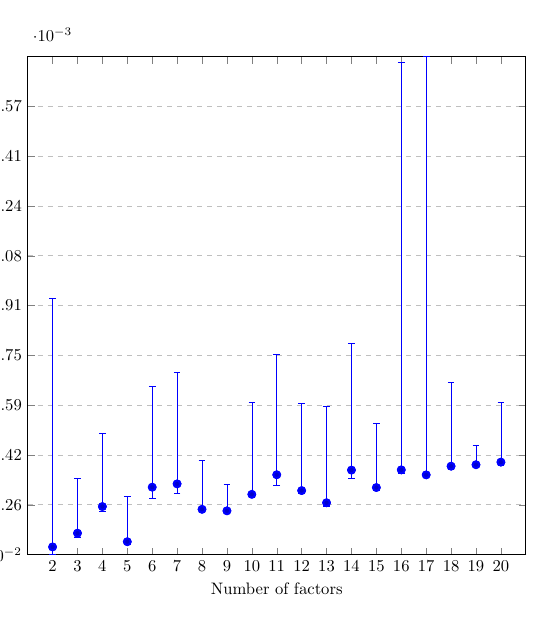
\begin{tikzpicture}[scale=0.6, trim axis left, trim axis right]
\begin{axis}[
    width=1\textwidth,
    height=1\textwidth,
    xlabel={Number of factors},
    ylabel={Time taken (s)},
    xmin=1.0, xmax=21.0,
    ymin=9.4e-05, ymax=0.001735,
    xticklabels={2, 3, 4, 5, 6, 7, 8, 9, 10, 11, 12, 13, 14, 15, 16, 17, 18, 19, 20},
    xtick={2, 3, 4, 5, 6, 7, 8, 9, 10, 11, 12, 13, 14, 15, 16, 17, 18, 19, 20},
    ytick={9.4e-05, 0.0002581, 0.0004222, 0.0005863, 0.0007504, 0.0009145, 0.0010786, 0.0012427, 0.0014068, 0.0015709},
    ymajorgrids=true,
    grid style=dashed,
]

\addplot+[
    blue,
    very thick,
    forget plot,
    only marks
    ]
    plot[
    very thick,
    error bars/.cd,
    y dir=plus,
    y explicit
    ]
    table[x=x,y=y,y error expr=\thisrow{y-max}] {
    x    y    y-max
    11	0.000356982894737	0.000398017105263
10	0.000292532894737	0.000304467105263
13	0.00026485	0.00031815
12	0.000304922368421	0.000287077631579
15	0.000314907894737	0.000210092105263
14	0.000372411842105	0.000418588157895
17	0.000356663157895	0.00137833684211
16	0.000373123684211	0.00134387631579
19	0.000390053947368	6.39460526316e-05
18	0.000385242105263	0.000274757894737
20	0.000398634210526	0.000197365789474
3	0.000164601315789	0.000180398684211
2	0.000119303947368	0.000819696052632
5	0.000136432894737	0.000150567105263
4	0.000252306578947	0.000239693421053
7	0.000327040789474	0.000365959210526
6	0.000316107894737	0.000332892105263
9	0.000238176315789	8.78236842105e-05
8	0.000243163157895	0.000161836842105

    };

\addplot+[
    blue,
    very thick,
    forget plot,
    only marks
    ]
    plot[
    very thick,
    error bars/.cd,
    y dir=plus,
    y explicit
    ]
    table[x=x,y=y,y error expr=\thisrow{y-min}] {
    x    y    y-min
    11	0.000356982894737	-3.39828947368e-05
10	0.000292532894737	-9.53289473685e-06
13	0.00026485	-1.185e-05
12	0.000304922368421	-9.92236842105e-06
15	0.000314907894737	-7.90789473684e-06
14	0.000372411842105	-2.64118421053e-05
17	0.000356663157895	-9.66315789473e-06
16	0.000373123684211	-1.21236842105e-05
19	0.000390053947368	-7.05394736842e-06
18	0.000385242105263	-9.24210526316e-06
20	0.000398634210526	-9.63421052632e-06
3	0.000164601315789	-1.46013157895e-05
2	0.000119303947368	-2.53039473684e-05
5	0.000136432894737	-8.43289473684e-06
4	0.000252306578947	-1.43065789474e-05
7	0.000327040789474	-3.00407894737e-05
6	0.000316107894737	-3.61078947368e-05
9	0.000238176315789	-6.17631578947e-06
8	0.000243163157895	-7.16315789474e-06

    };

\end{axis}
\end{tikzpicture}
\vspace{-0.3cm}
\caption{Small primes}\label{fig:TrialDivisionsmallprimesfactors}
\end{figure}



\begin{figure}[H]
\centering
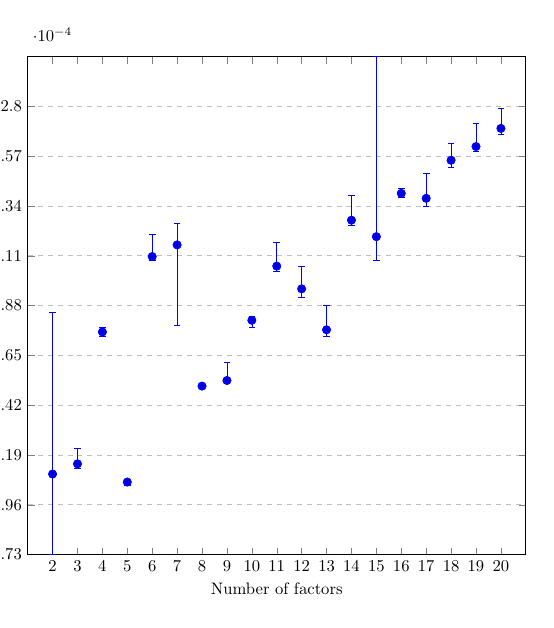
\begin{tikzpicture}[scale=0.6, trim axis left, trim axis right]
\begin{axis}[
    width=1\textwidth,
    height=1\textwidth,
    xlabel={Number of factors},
    ylabel={Time taken (s)},
    xmin=1.0, xmax=21.0,
    ymin=7.3e-05, ymax=0.000303,
    xticklabels={2, 3, 4, 5, 6, 7, 8, 9, 10, 11, 12, 13, 14, 15, 16, 17, 18, 19, 20},
    xtick={2, 3, 4, 5, 6, 7, 8, 9, 10, 11, 12, 13, 14, 15, 16, 17, 18, 19, 20},
    ytick={7.3e-05, 9.6e-05, 0.000119, 0.000142, 0.000165, 0.000188, 0.000211, 0.000234, 0.000257, 0.00028},
    ymajorgrids=true,
    grid style=dashed,
]

\addplot+[
    blue,
    very thick,
    forget plot,
    only marks
    ]
    plot[
    very thick,
    error bars/.cd,
    y dir=plus,
    y explicit
    ]
    table[x=x,y=y,y error expr=\thisrow{y-max}] {
    x    y    y-max
    11	0.0002062	1.08e-05
10	0.0001812	1.8e-06
13	0.0001768	1.12e-05
12	0.0001957	1.03e-05
15	0.0002198	8.32e-05
14	0.0002274	1.16e-05
17	0.0002375	1.15e-05
16	0.0002398	2.2e-06
19	0.0002614	1.06e-05
18	0.0002551	7.9e-06
20	0.0002698	9.2e-06
3	0.0001149	7.1e-06
2	0.0001102	7.48e-05
5	0.0001065	5e-07
4	0.0001758	2.2e-06
7	0.000216	1e-05
6	0.0002106	1.04e-05
9	0.0001534	8.6e-06
8	0.0001508	1.2e-06

    };

\addplot+[
    blue,
    very thick,
    forget plot,
    only marks
    ]
    plot[
    very thick,
    error bars/.cd,
    y dir=plus,
    y explicit
    ]
    table[x=x,y=y,y error expr=\thisrow{y-min}] {
    x    y    y-min
    11	0.0002062	-2.2e-06
10	0.0001812	-3.2e-06
13	0.0001768	-2.8e-06
12	0.0001957	-3.7e-06
15	0.0002198	-1.08e-05
14	0.0002274	-2.4e-06
17	0.0002375	-3.5e-06
16	0.0002398	-1.8e-06
19	0.0002614	-2.4e-06
18	0.0002551	-3.1e-06
20	0.0002698	-2.8e-06
3	0.0001149	-1.9e-06
2	0.0001102	-3.72e-05
5	0.0001065	-1.5e-06
4	0.0001758	-1.8e-06
7	0.000216	-3.7e-05
6	0.0002106	-1.6e-06
9	0.0001534	-1.4e-06
8	0.0001508	-8e-07

    };

\end{axis}
\end{tikzpicture}
\vspace{-0.3cm}
\caption{Small primes, modified algorithm}\label{fig:TrialDivisionsmallprimes(modified:True)factors}
\end{figure}



The largest benchmarks made are shown in the two figures below - for the unmodified and modified algorithm respectively.


\begin{figure}[H]
\centering
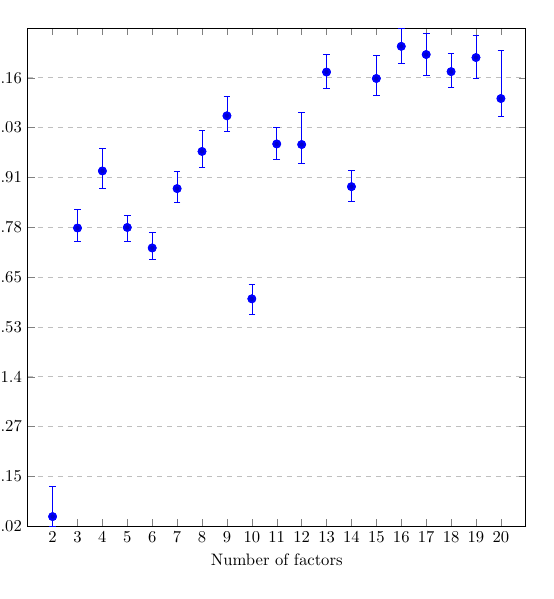
\begin{tikzpicture}[scale=0.6, trim axis left, trim axis right]
\begin{axis}[
    width=1\textwidth,
    height=1\textwidth,
    xlabel={Number of factors},
    ylabel={Time taken (s)},
    xmin=1.0, xmax=21.0,
    ymin=1.01826, ymax=2.287249,
    xticklabels={2, 3, 4, 5, 6, 7, 8, 9, 10, 11, 12, 13, 14, 15, 16, 17, 18, 19, 20},
    xtick={2, 3, 4, 5, 6, 7, 8, 9, 10, 11, 12, 13, 14, 15, 16, 17, 18, 19, 20},
    ytick={1.01826, 1.1451589, 1.2720578, 1.3989567, 1.5258556, 1.6527545, 1.7796534, 1.9065523, 2.0334512, 2.1603501},
    ymajorgrids=true,
    grid style=dashed,
]

\addplot+[
    blue,
    very thick,
    forget plot,
    only marks
    ]
    plot[
    very thick,
    error bars/.cd,
    y dir=plus,
    y explicit
    ]
    table[x=x,y=y,y error expr=\thisrow{y-max}] {
    x    y    y-max
    11	1.9919114	0.0415456
10	1.59734733333	0.0360946666667
13	2.17506696667	0.0449480333333
12	1.9904225	0.0819875
15	2.1586458	0.0591132
14	1.8831095	0.0412595
17	2.2197465	0.0536575
16	2.24052783333	0.0467211666667
19	2.21200643333	0.0571895666667
18	2.1760707	0.0471053
20	2.10760823333	0.123275766667
3	1.77776056667	0.0463764333333
2	1.04261126667	0.0767157333333
5	1.7791179	0.0317951
4	1.92306296667	0.0577200333333
7	1.87813433333	0.0443016666667
6	1.726933	0.040735
9	2.06360606667	0.0484439333333
8	1.9727841	0.0537149

    };

\addplot+[
    blue,
    very thick,
    forget plot,
    only marks
    ]
    plot[
    very thick,
    error bars/.cd,
    y dir=plus,
    y explicit
    ]
    table[x=x,y=y,y error expr=\thisrow{y-min}] {
    x    y    y-min
    11	1.9919114	-0.0391004
10	1.59734733333	-0.0387133333333
13	2.17506696667	-0.0424969666667
12	1.9904225	-0.0487505
15	2.1586458	-0.0421148
14	1.8831095	-0.0380765
17	2.2197465	-0.0525455
16	2.24052783333	-0.0434108333333
19	2.21200643333	-0.0531074333333
18	2.1760707	-0.0404237
20	2.10760823333	-0.0449892333333
3	1.77776056667	-0.0330955666667
2	1.04261126667	-0.0243512666667
5	1.7791179	-0.0357919
4	1.92306296667	-0.0448219666667
7	1.87813433333	-0.0348033333333
6	1.726933	-0.028244
9	2.06360606667	-0.0405510666667
8	1.9727841	-0.0399171

    };

\end{axis}
\end{tikzpicture}
\vspace{-0.3cm}
\caption{Larger primes}\label{fig:TrialDivisionLargerprimesfactors}
\end{figure}



\begin{figure}[H]
\centering
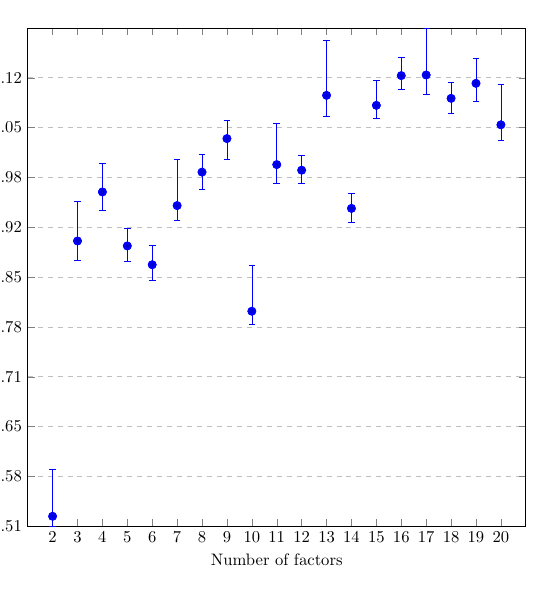
\begin{tikzpicture}[scale=0.6, trim axis left, trim axis right]
\begin{axis}[
    width=1\textwidth,
    height=1\textwidth,
    xlabel={Number of factors},
    ylabel={Time taken (s)},
    xmin=1.0, xmax=21.0,
    ymin=0.511378, ymax=1.185382,
    xticklabels={2, 3, 4, 5, 6, 7, 8, 9, 10, 11, 12, 13, 14, 15, 16, 17, 18, 19, 20},
    xtick={2, 3, 4, 5, 6, 7, 8, 9, 10, 11, 12, 13, 14, 15, 16, 17, 18, 19, 20},
    ytick={0.511378, 0.5787784, 0.6461788, 0.7135792, 0.7809796, 0.84838, 0.9157804, 0.9831808, 1.0505812, 1.1179816},
    ymajorgrids=true,
    grid style=dashed,
]

\addplot+[
    blue,
    very thick,
    forget plot,
    only marks
    ]
    plot[
    very thick,
    error bars/.cd,
    y dir=plus,
    y explicit
    ]
    table[x=x,y=y,y error expr=\thisrow{y-max}] {
    x    y    y-max
    11	1.00055786667	0.0557551333333
10	0.802164633333	0.0627623666667
13	1.09425033333	0.0750086666667
12	0.9929817	0.0201843
15	1.0807066	0.0343404
14	0.9413146	0.0206874
17	1.12181526667	0.0635667333333
16	1.12097466667	0.0249823333333
19	1.11051936667	0.0334966333333
18	1.09022053333	0.0217664666667
20	1.0544286	0.0550564
3	0.8972128	0.0534252
2	0.524697	0.063058
5	0.890506533333	0.0243284666667
4	0.9635399	0.0381631
7	0.945086366667	0.0620626333333
6	0.865081966667	0.0259950333333
9	1.0357376	0.0243904
8	0.9903779	0.0238771

    };

\addplot+[
    blue,
    very thick,
    forget plot,
    only marks
    ]
    plot[
    very thick,
    error bars/.cd,
    y dir=plus,
    y explicit
    ]
    table[x=x,y=y,y error expr=\thisrow{y-min}] {
    x    y    y-min
    11	1.00055786667	-0.0248278666667
10	0.802164633333	-0.0175326333333
13	1.09425033333	-0.0285023333333
12	0.9929817	-0.0184037
15	1.0807066	-0.0175756
14	0.9413146	-0.0194696
17	1.12181526667	-0.0267452666667
16	1.12097466667	-0.0178896666667
19	1.11051936667	-0.0242003666667
18	1.09022053333	-0.0202425333333
20	1.0544286	-0.0209746
3	0.8972128	-0.0261558
2	0.524697	-0.013319
5	0.890506533333	-0.0209495333333
4	0.9635399	-0.0248959
7	0.945086366667	-0.0196413666667
6	0.865081966667	-0.0205139666667
9	1.0357376	-0.0279266
8	0.9903779	-0.0226549

    };

\end{axis}
\end{tikzpicture}
\vspace{-0.3cm}
\caption{Larger primes, modified algorithm}\label{fig:TrialDivisionLargerprimes(modified:True)factors}
\end{figure}


Overall the unmodified algorithm seen in figure \ref{fig:TrialDivisionLargerprimesfactors} seem to take twice as long as the modified algorithm shown in figure \ref{fig:TrialDivisionLargerprimes(modified:True)factors}.

The rest of the data collected on the Trial Division algorithm can be found in the appendix \ref{trialdivisionplots}.